\section{Elicitation of requirements}
\label{sec:obtainingreq}

The customer did not provide a distinct set of specifications when the project first started. Instead, the team was provided with a general idea and a list of concepts that the customer requested. These concepts are shown as a set of prioritized steps in figure~\ref{fig:roadmap}, starting with ''Awareness of own consumption''. It was up to the team to produce a list of functional requirements that was later be approved by customer.

\begin{figure}[H]
\centering
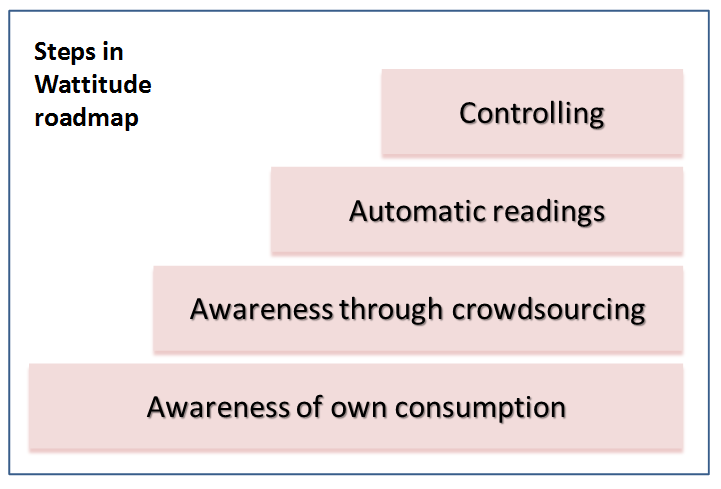
\includegraphics[height=0.37\textheight]{ch/specification/fig/roadmap.png}
\caption{Roadmap for Wattitude functionality}
\label{fig:roadmap}
\end{figure}

The core requirements were:
\begin{itemize}
\item The app should be user friendly and simple, so that anyone could measure their energy consumption. This was to be done preferably per device. 
\item The users should be able to share their energy consumption and production with their friends on Facebook. 
\item The concept of \gls{gamification} should be included into the app by allowing the users to compete with each other on saving and/or producing the most energy. 
\item The finished product should include a user manual and complete technical documentation.
\end{itemize}

A complete list of all requirements can be found in table~\ref{tab:funcReq}.
\noindent To measure the user's energy consumption per device, the team needed a hardware device. Optimally, such a device transmits  data either via Wifi, Bluetooth, or another form of wireless communication protocol.

Due to time restrictions, the requirement of having hardware monitoring and control over each individual device was deemed optional, and only to be attempted if the team had enough time. After the initial project planning and preliminary work, it became clear that this was to time consuming. The team and customer agreed to remove these requirements. 

However, the team agreed to do research on possible hardware solutions provided by the customer. This was done to ease integration in future development. See chapter~\ref{sec:further} for more information about further development. In addition to the requirements described in section~\ref{sec:functionalReq} and~\ref{sec:nonFunctionalReq}, the customer wanted a user manual for the app and technical documentation. These can be found in appendix~\ref{sec:userManual} and~\ref{sec:technicalDocumentation}.
